% iot_crop_growth.tex - Aplicaciones de IoT para la mejora de cultivos
\documentclass[10pt, twocolumn]{article}
%\documentclass[10pt]{report}

% ----------------------------------------------------- PAQUETES ----------------------------------------------------- %
% Lista de paquetes utilizados
\usepackage[spanish, mexico]{babel}
\usepackage[utf8]{inputenc}
\usepackage[T1]{fontenc}
\usepackage{lmodern}
\usepackage{graphicx}

\begin{document}

% ----------------------------------------------------- TÍTULO ----------------------------------------------------- %
% Propuestas: 
% - Internet de las Cosas y el crecimiento de cultivos: una revisión sistemática
% - Internet de las Cosas y el crecimiento apresurado de cultivos: una revisión sistemática
% - Internet de las Cosas y la agricultura: una revisión sistemática
% - Aplicaciones de IoT para la mejora de cultivos
\title{\textbf{Aplicaciones de IoT para la mejora de cultivos}}
\author{Freddy Íñiguez López\\
	Centro de Investigación en Matemáticas, A.C.,\\
	Zacatecas, México,\\
	\texttt{freddy.iniguez@cimat.mx}}
\date{Diciembre 2015}
\maketitle

% ----------------------------------------------------- ABSTRACT ----------------------------------------------------- %
\begin{abstract}
% 	- Context
% 	- Objectives
% 	- Methods
% 	- Results
% 	- Conclusions
[En desarrollo]
\end{abstract}
\paragraph{}
\textbf{Keywords} Internet de las Cosas | IoT | Agricultura | Sobrepoblación | Sustentabilidad

% ----------------------------------------------------- INTRODUCCIÓN ----------------------------------------------------- %
\section{INTRODUCCIÓN}
\paragraph{[En desarrollo]}
%\paragraph{[En desarrollo] \\ Los resultados obtenidos de esta revisión sistemática pretenden servir como base para la investigación de técnicas de Internet de las Cosas que ayuden a determinar las condiciones climáticas y de crecimiento para cierto cultivo y posteriormente desarrollar un modelo probabilístico que ayude a los agricultores y empresas de cultivos a mantener las mejores condiciones para un crecimiento óptimo y apresurado de sus cultivos. \\ Además, se tiene una problemática grave: actualmente ciertas zonas en el mundo están pasando por una deficiencia en la producción de sus cultivos, debido a que los nutrientes del suelo se están agotando, lo que promueve un crecimiento deficiente de los cultivos. De tal manera, si se lograra incrementar la producción de determindo cultivo con la propuesta de sistema de inferencia sobre las condiciones ambientales de un cultivo que se propone en el presente documento, ¿cuál sería el impacto con respecto al suelo? o ¿de qué manera se lograría esta propuesta?}

%\paragraph{Este documento solo se basa en la recopilación de artículos relacionados con sistemas de producción agrícola basados en Internet de las Cosas, específicamente en la manera en la que estos sistemas de producción agrícola obtienen las características ambientales y de crecimiento de un determinado cultivo. \\ ¿Cómo hacerlo de manera SUSTENTABLE? ¿Cómo hacerlo de manera AMIGABLE PARA EL AMBIENTE? Son dos incógnitas que quedan como trabajos futuros.}

% ----------------------------------------------------- REVISIÓN SISTEMÁTICA ----------------------------------------------------- %
% Etapa de la planificación de la revisión sistemática.
\section{REVISIÓN SISTEMÁTICA}
\paragraph{Esta sección contiene el detalle de las actividades desarrolladas correspondientes a la fase de planeación de la revisión sistemática. De tal manera, se muestra el planteamiento de la pregunta de investigación, en torno a la cual giran todas las demás actividades de la revisión sistemática, se detalla la estrategia a seguir para la recopilación de los estudios primarios y se muestra la definición de los criterios de inclusión y exclusión, los cuáles serán útiles al momento de realizar el filtro de los estudios primarios.}

\subsection{Antecedentes}
% El razonamiento de la revisión
% Problema 0: Sobrepoblación
\paragraph{A comienzos de los años 1800, la humanidad celebraba un gran acontecimiento: nos había tomado cerca de 250,000 años para llegar a ser 1,000,000,000 de personas en el mundo. Sin embargo, a partir de la revolución industrial, el crecimiento de la población fue en aumento de manera descontrolada. El segundo billón de personas llego apenas después de 127 años, en 1928. El tercer billón llegó en 1961, luego de 33 años. Para el cuarto billón de personas se necesitaron 14 años. Para 1988, celebrábamos el haber alcanzado los 5 billones de personas en el mundo. Tiempo después, de manera menos exponencial, bastaron 12 años para alcanzar la cifra de los 6 y 7 billones de personas, en el año 2000 y 2012 respectivamente. Para el primero de julio de 2015, se estimó que habitábamos en nuestro planeta tierra 7.349 billones de personas, acontecimiento que ya no celebramos de manera tan amena dadas las condiciones de inseguridad, pobreza, hambruna, problemas de salud, entre tantas más que vivimos.}

% Problema 1: Mayor demanda de comida
% Problema 2: Condiciones climáticas afectan cultivos
\paragraph{De acuerdo con el reporte del panel para la sustentabilidad global de la Secretaría General de las Naciones Unidas, para el año 2030 la población requerirá de por lo menos 50\% más comida, 45\% más energía y 30\% más agua~\cite{globalsustainabilityreport}. Hablando específicamente de la situación alimenticia a futuro, se estima que para el año 2050 la demanda de comida crezca un 70 por ciento con respecto a la demanda actual. \\ Además, cabe mencionar que las condiciones climáticas que vivimos hoy en día son producto del cambio climático y del calentamiento global, problemas ambientales que si se presentan en condiciones extremas pueden llegar a afectar a la mayoría de los cultivos, empeorando la situación del suministro de comida.}

% Problema 3: Uso excesivo de herbicidas
\paragraph{Y por si las condiciones climáticas fueran ya un problema grave que afecta el crecimiento de los cultivos, es importante hacer notar que utilizar herbicidas, fertilizantes y plaguicidas afectan negativamente tanto al ambiente como a ciertos animales, especialmente disminuye la capacidad y nutrientes del suelo. Lo anterior se convierte en un problema recursivo, ya que en el afán de incrementar la producción de cultivos, se hace uso excesivo de herbicidas, lo que daña al ambiente y a las condiciones nutrimentales del suelo, lo que impide que los cultivos se desarrollen adecuadamente.}

% Motivación de la investigación
\paragraph{Por tal razón, es de vital importancia que se desarrollen estrategias que ayuden a combatir esta serie de problemas que se preveen para el futuro. En lugar de utilizar herbicidas de una manera descontrolada, se deben implementar estrategias para que los campos de cultivo generen una mayor cantidad de alimento, o que puedan generar la misma cantidad de alimento pero tener más temporadas de producción al año, de una manera sustentable y que sea amigable con el ambiente y con el suelo.}

% Propuesta:
% 1) Obtener condiciones de desarrollo y ambientales de los cultivos, utilizando IoT, (obtener condiciones de los cultivos)
% 2) Desarrollo de modelo propabilístico que ayude a mantener las estables y óptimas las condiciones de crecimiento de los cultivos, haciendo inferencias para con los cambios de clima o desastres naturales que pudieran afectar, (desarrollo de modelo que mantenga estable y óptimo su crecimiento)
% 3) Investigación en agro-industria para modelo de desarrollo de cultivos sustentable, (de manera sustentable) y
% 4) Investigación en agro-industria para modelo de desarrollo acelerado de cultivos (para producir más).
\paragraph{El presente trabajo de investigación forma parte de una de las primeras etapas para la obtención de un nuevo modelo de producción agrícola sustentable, el cual es una propuesta que da solución al problema de demanda de alimento en un futuro. \\ Se cree que la propuesta completa podría dividirse en cuatro etapas, las cuales se describen de manera general a continuación:}
\begin{enumerate}
	\item{Obtener condiciones ambientales y de desarrollo de los cultivos, utilizando técnicas de Internet de las Cosas,}
	\item{Desarrollo de un modelo probabilístico que ayude a mantener estables y óptimas las condiciones de crecimiento de los cultivos, haciendo inferencias para con los cambios de clima o temporadas que pudieran afectar su crecimiento,}
	\item{Investigación en agro-industria para desarrollo de modelo de cultivos sustentable, y}
	\item{Investigación en agro-industria para acelerar el crecimiento de los cultivos.}
\end{enumerate}
\paragraph{De tal manera, el presente trabajo se enfoca en la primera etapa de esta propuesta, para lo cual es necesario conocer las estrategias, técnicas y métodos actuales que se utilizan en la agricultura para la obtención de las características ambientales de los cultivos utilizando técnicas de Internet de las Cosas.}

\subsection{Objetivos}
\subsubsection{Objetivo general}
\begin{itemize}
	\item{Conocer las estrategias, métodos o procedimientos basados en Internet de las Cosas que existen en la actualidad para determinar las características ambientales y de crecimiento de los cultivos.}
\end{itemize}
\subsubsection{Objetivos específicos}
\begin{itemize}
	\item{Definir la motivación de la investigación.}
	\item{Concretar objetivos y pregunta de investigación.}
	\item{Definir palabras clave, cadenas de búsqueda y criterios de exclusión e inclusión.}
	\item{Aplicar las búsquedas para la obtención de artículos.}
	\item{Aplicar los criterios de exclusión e inclusión para la obtención de estudios primarios.}
	\item{Realizar un análisis a los estudios primarios obtenidos.}
	\item{Obtener resultados, conclusiones y presentarlos.}
\end{itemize}

\subsection{Pregunta de investigación}
% Las preguntas que la investigación pretende responder.
% El objetivo de una revisión sistemática es encontrar la mayor cantidad de estudios primarios como sea posible, relacionados con una pregunta de investigación usando una estrategia de búsqueda imparcial.
\paragraph{Con la intención de conocer las estrategias, métodos o procedimientos que existen en la actualidad para determinar las características ambientales y de crecimiento de los cultivos, se desarrolla la siguiente pregunta de investigación, la cual a su vez servirá de guía para la definición de las demás actividades de la revisión sistemática.}
% Población: granjas y agricultores.
% Intervención: Tecnologías/herramientas/métodos/metodologías de Internet de las Cosas.
% Comparación: las condiciones climáticas para el crecimiento óptimo de cultivos.
% Salidas: ayudar a tener condiciones óptimas en los cultivos.
% Contexto:
\begin{itemize}
	\item{¿Qué herramientas, estrategias o métodos enfocados al Internet de las Cosas existen para determinar las características ambientales y de crecimiento de los cultivos?}
\end{itemize}

\subsection{Estrategia}
% Estrategia que se utilizará para la búsqueda de estudios primarios incluyendo términos de búsqueda y los recursos en los que serán buscados.
% Los recursos incluyen bibliotecas digitales, revistas específicas y actas de congresos.
\paragraph{Para la búsqueda de estudios primarios es necesario definir las cadenas o términos de búsqueda así como también las fuentes en donde serán aplicadas estas búsquedas, como revistas científicas, bases de datos, libros electrónicos u otros recursos libres y bibliotecas. \\ De tal manera, se muestran a continuación las cadenas de búsqueda a aplicar.}
\begin{enumerate}
	\item{Internet of Things OR IoT AND crop AND growth}
	\item{Internet of Things OR IoT AND agriculture}
	\item{Internet of Things OR IoT AND food AND production}
	% Cadenas de búsqueda añadidas:
	\item{Internet of Things OR IoT AND sustainable AND agriculture}
	\item{Internet of Things OR IoT AND sustainable AND crop}
	\item{Internet of Things OR IoT AND predictable AND model AND agriculture}
	% Cadenas de búsqueda descartadas:
	%\item{Internet of Things OR IoT AND rapid crop growth}
	%\item{Internet of Things OR IoT AND accelerated crop growth}
\end{enumerate}
\paragraph{Y para el caso de las fuentes que serán utilizadas se muestran a continuación aquellas seleccionadas por su alto grado de relevancia en el campo científico.}
\begin{itemize}
	\item{ACM Digital Library}
	\item{IEEE Explore}
	\item{SpringerLink}
	\item{Elsevier Science}
	\item{AGRIS: International Information System for the Agricultural Science and Technology}
\end{itemize}
\paragraph{Cabe mencionar que la última de estas fuentes se refiere a un buscador especializado en temas de agricultura que pone a disposición la Organización de Agricultura y Comida de las Naciones Unidas. Esto le agrega un valor al estudio, ya que dentro de esta base de datos se pudiera encontrar información muy importante y primaria para cumplir los objetivos que persigue esta revisión sistemática.}

\subsection{Criterios de selección de estudios}
% Los criterios de selección de estudios se utilizan para determinar cuáles estudios son incluídos y cuáles son excluídos de la revisión sistemática.
% Es muy útil para pilotear los criterios de selección en un subconjunto de estudios primarios.
\paragraph{Una vez que se apliquen las cadenas de búsqueda y se obtenga un conjunto de estudios, será necesario realizar una evaluación a cada uno y categorizarlos de acuerdo al tipo de estudio del que se trate. Para ello se deben definir criterios para la selección de estudios, que para el caso de la presente revisión sistemática se detallan a continuación.}
% Criterios de inclusión
\paragraph{Se incluirán en la revisión sistemática aquellos estudios que sean o que cumplan con las siguientes características:}
\begin{itemize}
	\item{Técnicas, métodos o herramientas de Internet de las Cosas para medir las condiciones climáticas de un cultivo.}
	\item{Aplicaciones del Internet de las Cosas en la agricultura.}
	\item{Sistemas o aplicaciones de producción agrícola basado en Internet de las Cosas.}
	\item{Sistemas o aplicaciones de distribución y producción de cultivos basado en Internet de las Cosas.}
	\item{Ecosistemas de agricultura basado en Internet de las Cosas.}
	\item{Sistemas o aplicaciones de monitoreo de cultivos basado en Internet de las Cosas.}
	\item{Sistemas de trazabilidad de cultivos basado en Internet de las Cosas.}
	\item{Marcos de trabajo para el monitoreo de cultivos basado en Internet de las Cosas.}
	\item{Plataformas de monitoreo y control de cultivos basado en Internet de las Cosas.}
	\item{Modelos de aceleración de cultivos basado en Internet de las Cosas.}	
	\item{Investigaciones acerca de sistemas inteligentes de granjas basado en Internet de las Cosas.}
	\item{Sistemas o aplicaciones para la detección temprana de anomalías en el crecimiento de los cultivos.}
	\item{Sistemas o aplicaciones para la detección temprana de anomalías en el crecimiento de una especie determinada de cultivo.}
	\item{Investigaciones o sistemas inteligentes de granjas o \textit{smart farm} para la detección temprana de anomalías en el crecimiento de una especie determinada de cultivo.}
\end{itemize}
% Criterios de exclusión
\paragraph{Se excluirán de la revisión sistemática aquellos estudios que sean o que cumplan las siguientes características:}
\begin{itemize}
	\item{Técnicas, métodos o herramientas que midan las condiciones climáticas de un cultivo pero que éstas no se relacionen con técnicas de Internet de las Cosas.}
	\item{Aplicaciones del Internet de las Cosas para la gestión y control de sistemas agrícolas.}
	\item{Sistemas de producción agrícola tradicionales.}
	\item{Sistemas o aplicaciones de distribución y producción agrícola tradicionales.}
	\item{Investigaciones sobre sistemas inteligentes de granjas o \textit{smart farm} para la detección temprana de plagas.}
	\item{Investigaciones sobre enfermedades en los cultivos.}
	\item{Investigaciones sobre nuevas variedades de cultivos.}
	\item{Investigaciones sobre Internet de las Cosas.}
	\item{Investigaciones sobre agricultura.}
	\item{Estudios repetidos.}
\end{itemize}

\subsection{Procedimientos de selección de estudios}
% El protocolo debe describir cómo serán aplicados los criterios de selección. Por ejemplo, cuántos asesores evaluarán cada estudio primario prospecto.
% Cómo serán resueltos los desacuerdos entre asesores.
\paragraph{El procedimiento para la selección de estudios primarios se concentrará en la evaluación de los criterios de exclusión e inclusión descritos en la sección anterior. Es decir, primeramente se comparará cada artículo resultado de la búsqueda con cada uno de los criterios de exclusión en el orden en el que estos aparecen. Al momento en el que alguno de los criterios de exclusión coincida con el artículo, éste se descartará y se procederá a evaluar el siguiente artículo. Si al agotar cada uno de los criterios de exclusión el artículo no ha sido descartado, se procede a compararlo con cada uno de los criterios de inclusión. \\ De igual manera, el artículo será comparado con cada uno de los criterios de inclusión conforme fueron escritos anteriormente. En el momento en el que el artículo coincida con algún criterio de inclusión, se procederá a conservar dicho artículo y se continuará evaluando los artículos restantes. En todo caso, si al agotar la lista completa de criterios de inclusión el artículo no coincidió con alguno, éste será conservado temporalmente y se discutirá con el asesor la permanencia o descarte de este artículo.}

\subsection{Estrategia de extracción de datos}
% Ésta define cómo la información requerida de cada estudio primario será obtenida.
% Si los datos requieren manipulación o suposiciones e inferencias, el protocolo debe especificar un proceso de validación apropiado.
\paragraph{Una vez que los criterios de inclusión y exclusión hayan sido aplicados, es necesario realizar un análsis a los estudios primarios con la intención de obtener la información requerida para contestar la pregunta de investigación y cumplir con los objetivos. \\ En el caso de este trabajo, la pregunta de investigación se concentra en conocer las técnicas, herramientas y métodos para la obtención de las características ambientales y de crecimiento de los cultivos. \\ Sin embargo, la descripción de un método puede llegar a ser algo extensa como para que se mencione de manera explícita, sino más bien el autor dará una descripción detallada del método, los protocolos utilizados y la manera en la que opera. Por tanto, el proceso para obtener esta información será el siguiente:}
\begin{enumerate}
	\item{Lectura del resumen o abstract en busca del nombre del método, técnica o herramienta utilizada para la obtención de las características ambientales de los cultivos.}
	\item{Lectura de la metodología utilizada, descripción de la arquitectura propuesta, descripción del diseño y partes que componen el método, sección de implementación o sección crítica y principal de cada artículo, con la intención de identificar el protocolo y detalle de operación del método, técnica o herramienta descrita.}
\end{enumerate}

\subsection{Síntesis de datos extraídos}
% Definir una estrategia para síntesis de datos.
% Esta estrategia debe aclarar si se pretende aplicar un meta-análisis formal o no, y en caso de aplicarse, qué técnicas se aplicarán.
\paragraph{La información relevante de cada uno de los artículos debe estar enfocada en responder a la pregunta de investigación de una manera sencilla, pero a la vez detallada en caso de que se requiera profundizar en el tema. Por tanto, la información requerida para responder a la pregunta de investigación debe ser fácil de identificar para cada uno de los artículos. \\ De esta manera, se pretende recopilar en una tabla la siguiente información:}
\begin{itemize}
	\item{Nombre del artículo,}
	\item{Nombre del método, técnica o herramienta que se utiliza para la obtención de las condiciones ambientales y de crecimiento de los cultivos,}
	\item{Protocolo de comunicación utilizado,}
	\item{Descripción general del método, técnica o herramienta,}
	\item{Resultados obtenidos o factibilidad del método.}
\end{itemize}

\subsection{Estrategia de diseminación}
% Para quién serán importantes los resultados de la revisión sistemática.
% Planificar cómo será realizada la difusión de los resultados de la revisión sistemática.
\paragraph{Finalmente, los resultados de la presente revisión sistemática deberán sintetizar las distintas maneras en la que actualmente se obtienen las características ambientales y de crecimiento de ciertos cultivos, además de mencionar si estas técnicas y herramientas son factibles de implementar, o en todo caso cuáles son las dificultades que se tienen para hacer de este método una solución factible.}

% ----------------------------------------------------- METODOLOGÍA DE INVESTIGACIÓN ----------------------------------------------------- %
% Etapa de la ejecución de la revisión sistemática.
\section{EJECUCIÓN DE LA METODOLOGÍA}
\paragraph{En este capítulo se presentan los resultados obtenidos de la aplicación de las cadenas de búsquedas y de los criterios de inclusión y exclusión para la obtención de los estudios primarios, o lo que se refiere a la etapa de ejecución de la revisión sistemática.}

\subsection{Resultados de las búsquedas}
\paragraph{Toda vez que las cadenas de búsqueda han sido definidas, al igual que fuentes donde serán aplicadas las primeras y los criterios de inclusión y exclusión para la obtención de estudios primarios, se procede a realizar las búsquedas correspondientes. \\ Podemos ver que los resultados de las búsquedas han sido resumidos en una sola tabla (ver Tabla 1). En este caso, cabe mencionar que la búsqueda avanzada en algunas de las fuentes, como AGRIS y SpringerLink, no existía o no se podían especificar ciertos criterios, por lo que en algunos resultados se obtienen datos muy altos debido a que la cadena de búsqueda fue aplicada tal y como se definió.}
\begin{table}[b]
\centering
\begin{tabular}{|c|c|c|c|c|c|c|}
\hline
\multicolumn{1}{|c|}{\textbf{Fuente}} & \multicolumn{6}{c|}{\textbf{Cadenas de búsqueda}}                                                                                                                                                         \\ \hline
                                      & \multicolumn{1}{c|}{\textbf{1}} & \multicolumn{1}{c|}{\textbf{2}} & \multicolumn{1}{c|}{\textbf{3}} & \multicolumn{1}{c|}{\textbf{4}} & \multicolumn{1}{c|}{\textbf{5}} & \multicolumn{1}{c|}{\textbf{6}} \\ \hline
ACM                                   & 0                              & 4                              & 1                              & 1                              & 0                              & 0                              \\ \hline
IEEE                                  & 11                              & 81                              & 16                              & 10                              & 2                              & 0                              \\ \hline
SpringerLink                          & 2,363                              & 5,982                              & 9,616                         	     & 2,604                              & 1,397                              & 593                              \\ \hline
Elsevier                              & 1,459                              & 3,795                              & 6,356                              & 1,551                              & 850                              & 320                              \\ \hline
AGRIS                                 & 8,061                              & 743,172                              & 8,254                              & 1,651                              & 910                              & 1                              \\ \hline
\end{tabular}
\caption{Resultados de las búsquedas.}
\label{tabla:busquedas}
\end{table}

\paragraph{Cabe mencionar que para efectos de la presente revisión sistemática, solo se considerarán los artículos obtenidos de la fuente IEEE Explore, ya que se cuenta con una limitante de tiempo para concluir el presente. De esta manera, el resto de la ejecución de la revisión sistemática se basará en los 120 estudios obtenidos de la fuente IEEE Explore.}

\subsection{Obtención de estudios primarios}
\paragraph{Una vez que se han aplicado las cadenas de búsqueda y se han obtenido el conjunto de artículos, se procedió a realizar la aplicación de los criterios de inclusión y exclusión definidos para la presente revisión sistemática. \\ En primer lugar se utilizó el gestor de referencias Mendeley para incluir todos los resultados de la búsqueda (recordamos que solo se están considerando los resultados de la fuente IEEE Explore para con todas las cadenas de búsqueda). Una vez hecho esto, se procedió a comparar cada uno de los artículos con los criterios de inclusión y excusión, leyendo el título y abstract (y en algunas ocasiones la introducción) para luego determinar su permanencia o descarte en el conjunto de estudios primarios.}

\paragraph{Hecha la comparación de cada uno de los resultados de la búsqueda con los criterios de inclusión y exclusión definidos, se obtiene que de los 120 artículos iniciales se consideran como estudios primarios 46 de ellos.}

\subsection{Extracción de la información}
\paragraph{El proceso para extraer la información de los estudios primarios ha sido definido y se seguirá en esta etapa de la revisión sistemática. Primeramente, se crea una tabla que contiene los siguientes encabezados:}
\begin{itemize}
	\item{Nombre del artículo}
	\item{Método, técnica o herramienta}
	\item{Protocolo de comunicación utilizado}
	\item{Descripción general del método}
	\item{Resultados y factibilidad del método}
\end{itemize}
\paragraph{Posteriormente se comenzó a leer cada uno de los estudios primarios, completando los campos de la tabla anterior.}

% ----------------------------------------------------- RESULTADOS ----------------------------------------------------- %
% Etapa de reportar resultados de la revisión sistemática.
\section{RESULTADOS}
\paragraph{Como parte de los resultados encontrados tras analizar los estudios primarios productos de la presente revisión sistemática, podemos enlistarlos como sigue. Cabe mencionar una vez más que por la restricción del tiempo no se están considerando los resultados de todas las fuentes propuestas en la sección 2.4, ya que nos tomaría más tiempo del dispuesto hacer el filtrado y análisis de todos los resultados.}
\begin{itemize}
	\item{Como parte de la novedad y resultados obtenidos hasta el día de hoy, existen muchas aplicaciones en diferentes campos para el Internet de las Cosas. Específicamente lo es dentro del campo de la agricultura, ya sea para administrar sistemas de producción agrícolas, controlar sistemas de riego agrícolas, monitorear las condiciones ambientales y de crecimiento de los cultivos y hasta aplicaciones de sensibilización y moderamiento del desperdicio de comida.}
	\item{Se puede percibir una tendencia hacia la implementación de una arquitectura en tres capas, como se puede apreciar en la Figura 1. Primero se encuentra la capa de obtención de los datos o WSN. Posteriormente estos datos son coleccionados en un servidor o computador central llamado B/N para finalmente compartir los datos en la capa de aplicación.}
	\item{De la misma manera, existen dos tendencias para con las técnicas, herramientas y métodos utilizados para la obtención de las características ambientales y de crecimiento de los cultivos:}
	\begin{enumerate}
		\item{Creación de protocolos ad hoc basado en TCP, UDP.}
		\item{Utilización o creación de protocolos ad hoc basados en estándares abiertos como OpenIoT o ZigBee.}
	\end{enumerate}
	\item{En cuestión de la factibilidad de los métodos propuestos, la mayoría expone que son factibles por diferentes razones. Las más comunes son porque ahorran tiempo, dinero, facilitan la comunicación, mejoran la organización del sistema de producción y permiten compartir los resultados.}
\end{itemize}
\begin{figure}[!ht]
	\centering
	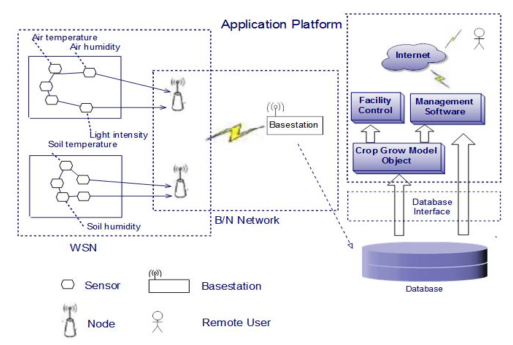
\includegraphics[scale=0.5]{common_architecture.png}
	\caption{Arquitectura típica encontrada.}
\end{figure}

% ----------------------------------------------------- CONCLUSIONES ----------------------------------------------------- %
\section{CONCLUSIONES}
\paragraph{El problema de la sobrepoblación se encuentra en una situación grave, en la que es posible observar algunas de sus consecuencias dentro de las áreas de pobreza, inseguridad, desempleo, problemas de salud, entre otros. Sin embargo, se prevee que esta serie de problemas se complique en un futuro, ya que los índices del crecimiento de la población indican que ésta seguirá creciendo, si bien de una manera menos descontrolada.}
\paragraph{El presente trabajo de invetigación se enfoca en la revisión sistemática de técnicas, herramientas y métodos existentes para la obtención de las características ambientales y de crecimiento de los cultivos, con la simple intención de conocer cuáles son los trabajos actuales, cuáles han sido sus ventajas y oportunidad y también para conocer las dificultades que se les han presentado.}

% ----------------------------------------------------- REFERENCIAS ----------------------------------------------------- %
\bibliographystyle{plain}
\bibliography{iot_crop_growth}

\end{document}